\subsection{Macaque V1 spontaneous and evoked activity separate along the predicted CV--sparseness axis}
\label{sec:cv_s_data}

We test whether macaque V1 activity occupies the predicted high-CV, high-sparseness region in the spontaneous--evoked contrast.  Throughout this section we use the lifetime CV ($\mathrm{CV}_L$, across trials per neuron) and lifetime sparseness ($S_L$); the per-trial population estimator ($\mathrm{CV}_P/S_P$) on the same dataset is shown in Supplementary Fig.~S3.

Analyzing simultaneous extracellular recordings from macaque V1 \cite{23}, individual neurons in the spontaneous state exhibit substantially higher lifetime variability and sparseness than in the stimulus-driven state (Fig.~\ref{fig:V1}C; per-neuron $\mathrm{CV}_L$ median $0.82$ vs.\ $0.63$, $\sim 30\%$ higher; $S_L$ median $0.40$ vs.\ $0.29$; paired across $N=159$ neurons).  Spontaneous activity thus occupies the high-$\mathrm{CV}_L$, high-$S_L$ region of the coding space, consistent with the Gibbs-manifold prediction that the resting state sits at high coding readiness within a tight metabolic budget.

The empirical $S$--CV relation follows the monotonic curve predicted by the algebraic identity (Fig.~\ref{fig:V1}D).  Because this identity is sampling-symmetric (it holds for $S$ and CV computed over any non-negative response samples), the V1 result confirms that spontaneous and evoked activity occupy different regions of the response-statistics coordinate system rather than constituting an independent test of Gibbs optimality, which would require independent metabolic-budget measurement.  The Vinje--Gallant bias-corrected Treves--Rolls sparseness \cite{20} simplifies, upon substituting $\mathrm{CV}=\sigma/\langle r\rangle$, to
\begin{equation}
S = \frac{1}{1 - 1/N}\,\frac{\mathrm{CV}^2}{\mathrm{CV}^2 + 1},
\label{eq:S-CV-identity}
\end{equation}
approaching $S = \mathrm{CV}^2/(\mathrm{CV}^2+1)$ for large $N$.  Simulated spike sequences with Poisson, Gaussian, and uniform ISI statistics trace the same identity (Supplementary Fig.~S2; Supp.~Sect.~2.1), confirming that this is a general statistical constraint of non-negative firing distributions.

Given that spontaneous activity accounts for a substantial fraction of cortical metabolic expenditure \cite{Raichle2001,Tomasi2013}, maintaining high $\mathrm{CV}_L$ in the resting state may serve to preserve coding capacity for rapid responses to unexpected stimuli without costly reorganization of activity statistics.  One interpretive caveat: the recordings were obtained under sufentanil anesthesia, which can elevate slow-wave activity and inflate spontaneous variability measurements.  The direction of the spontaneous--evoked contrast is qualitatively consistent with prior reports in awake preparations \cite{Jia2024variability}, but quantitative verification under awake, naturalistic conditions remains warranted.

\paragraph{Empirical noise-entropy fraction.}
The deterministic-encoding approximation $I(s;r)\approx H(r)$ used in the Gibbs derivation is an idealization.  Direct-Method estimation \cite{strong1998entropy} (Methods) on the V1/V2 recordings yields $\bar\rho \equiv H(r\mid s)/H(r) \approx 0.85$ (V1: $n=159$, IQR $[0.83,0.90]$; V2: $n=25$, $\bar\rho=0.81$), so $I\approx 0.15\,H$ rather than $I\approx H$ on this dataset, plausibly because of anesthesia and the limited drifting-grating ensemble (Supp.~Note ``Empirical noise-entropy fraction'').  This does not falsify the Gibbs derivation: $\rho$ is approximately uniform across neurons (V1 IQR width $0.06$), so $I=(1-\bar\rho)H$ rescales ICE by a state-independent multiplicative constant within the evoked condition, leaving the rank ordering and monotonic ICE--CV structure unchanged.  The rescaling applies only to within-evoked rank-order comparisons; spontaneous activity has no defined stimulus and $H$ is reported in coding-readiness units throughout (the spontaneous--evoked $H$ vs.\ $I$ gap is revisited in Fig.~\ref{fig:Gibbs-frontier}C).

\begin{figure*}
\centering
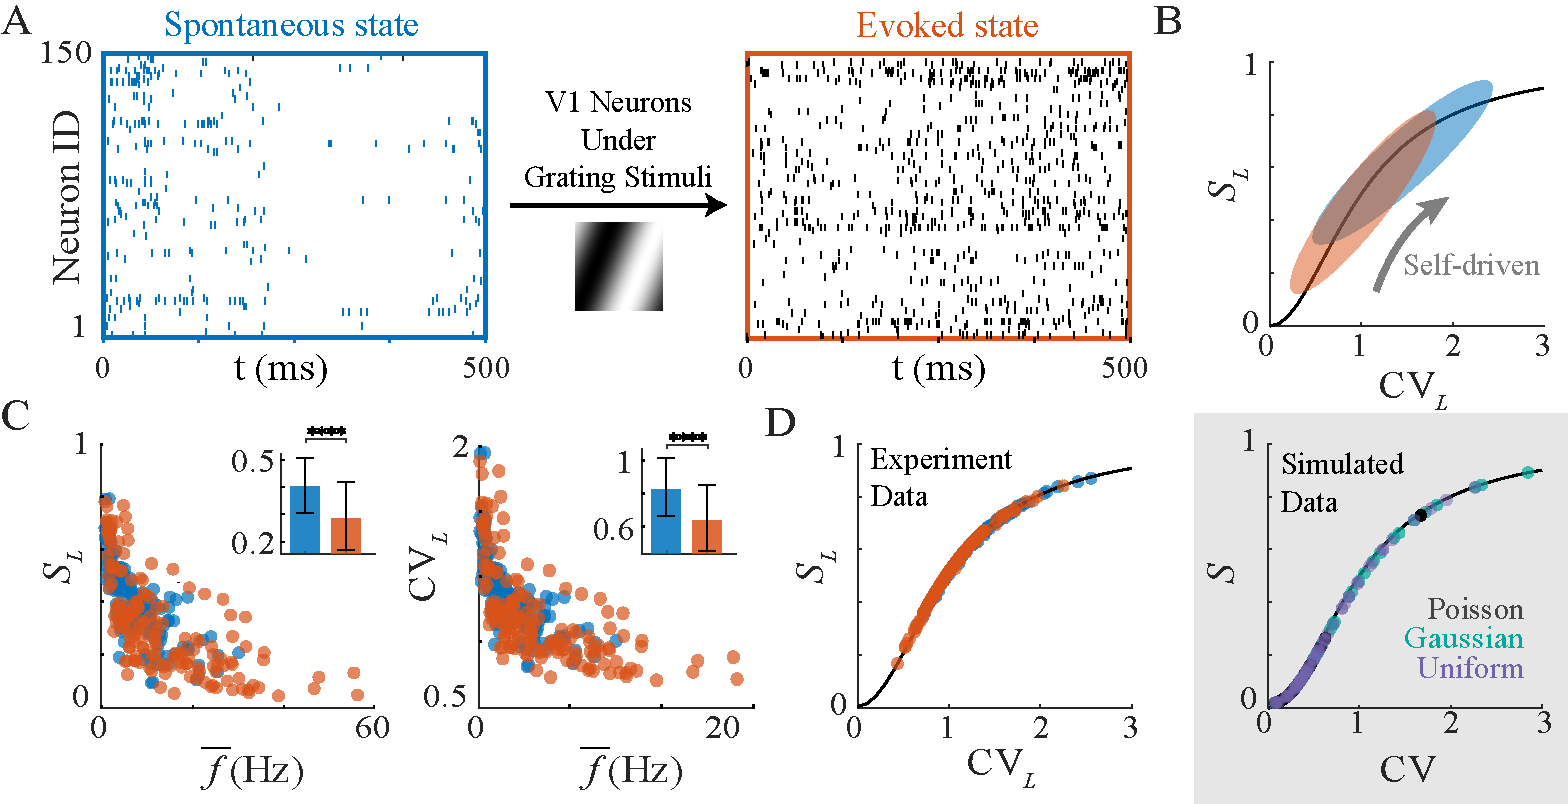
\includegraphics[scale=0.45]{figures/Figure2.pdf}
\caption{\textbf{Lifetime variability and sparseness of V1 neurons separate spontaneous from evoked states.}  $\mathrm{CV}_L$: lifetime coefficient of variation of a single neuron's firing rate across trials; $S_L$: Vinje--Gallant bias-corrected Treves--Rolls sparseness over the same per-neuron sample.  Each dot in C--D is one V1 neuron; spontaneous (blue), evoked (orange).  Dataset details in Methods; the complementary per-trial population view ($\mathrm{CV}_P$) is in Supplementary Fig.~S3.
(\textbf{A}) Representative raster plots of V1 neurons during a spontaneous (left) and evoked (right) trial.
(\textbf{B}) Schematic of the $S_L$--$\mathrm{CV}_L$ manifold for the two states.  Spontaneous points throughout this figure are in entropy/coding-readiness units, not measured stimulus information.
(\textbf{C}) $S_L$ (left) and $\mathrm{CV}_L$ (right) vs.\ mean firing rate.  Spontaneous neurons sit at higher $\mathrm{CV}_L$ and $S_L$ (median $\mathrm{CV}_L=0.82$, $S_L=0.40$) than evoked ($0.63$, $0.29$; paired across $N=159$ neurons; insets: $^{****}p<10^{-4}$).  Full statistics in Supplementary Table~S6.
(\textbf{D}) $S_L$--$\mathrm{CV}_L$ relation: V1 data (coloured) and the theoretical identity $S=\mathrm{CV}^2/(1+\mathrm{CV}^2)$ (black, Eq.~\ref{eq:S-CV-identity}); the relation holds for both states.  Inset: simulated spike sequences with Poisson, Gaussian, and uniform ISI statistics trace the same identity (also Supplementary Fig.~S2).}
\label{fig:V1}
\end{figure*}
